%!TEX root = main.tex

\section{Our adaptive-based broadcast algorithm for heterogeneous MANET's}

\subsection{Adaptation mechanism}

\raziel{
Lemma to prove the correctness of our adaptation mechanism. Plan of work:
\begin{itemize}
	\item write down lemma having broadcast messages as abstract as possible. Some consideration while writing lemma:
	\begin{itemize}
		\item the generalization of our claim will take place saying that our mechanism is valid when $A$ is the set of ALL existing broadcast algorithms and not when $A$ is just ONE set of protocols, as we do right now.
		%
		This can be mention as future work having a reasoning about what exactly is $A$ in this current version of the lemma.
		%
		 Q: How can we proof a lemma when $A$ refers to all existing broadcast protocols? (big question)
		\begin{itemize}
			\item Q: shall we have a taxonomy of broadcast algorithms in mind? ANSWER: say that we do.
			%
			Then, we must define that any $p \in O$ or $p \in N$ where $O$ refers to all overlay-based algorithms and $N$ is the set of non overlay-based algorithms; which is a valid generalization(I guess?)
			\item proof by induction over any $p_{i}$
			\item proof by contradiction over any $p_{i}$. $\exists p_{i} \in O$ that lost a message $M_{p_{j}}$, then find a bimodal value in data structures of $p_{i}$ OR an incorrect functioning in the way $p_{i}$ operates to show that a contradiction actually exists
		\end{itemize}
	\end{itemize}
	\item write down proof of lemma by contradiction
\end{itemize}
}

\begin{lemma}
	Let be $M_{p_{i}}$ a message and $p_{i}$ a broadcast protocol such that $p_{i} \in A$, where $A$ is a set of protocols. If a node $N$ receives $M_{p_{i}}$ while $p_{j}$ is in execution at $N$, then Algorithm~\ref{alg:adaptation_mechanism} translates $M_{p_{i}}$ into $M_{p_{j}}$ for being disseminated by $N$ using $p_{j}$.
\label{lemma:adapt_mech}
\end{lemma}

We need to guarantee that Algorithm~\ref{alg:adaptation_mechanism} does not drop any incoming message $M_{p_{i}}$ while a protocol $p_{j}$ is in execution on node $N$.
%
This potential loss of messages could take place only in line~\ref{alg:adaptation_mechanism:handle} or ~\ref{alg:adaptation_mechanism:emit} of Algorithm~\ref{alg:adaptation_mechanism}.
%
We avoid the case where there is a call of function $\AlgoHandle(\Ms)$ (line~\ref{alg:adaptation_mechanism:handle}, Algorithm~\ref{alg:adaptation_mechanism}), because our adaptation mechanism does not interfere with the way any protocol operates.
%
Thus, we offer a proof of lemma~\ref{lemma:adapt_mech} considering the case where the message translation take place (line~\ref{alg:adaptation_mechanism:emit}, Algorithm~\ref{alg:adaptation_mechanism}), as follows:

\textbf{Proof.}
Let $M_{p_{i}}$ be a message that was successfully received by node $N$ for the first time, but its translation into message $M_{p_{j}}$ was not forwarded.
%
Given that we want to validate the message translation procedure, not unexpectedly, protocol $p_{j}$ is in execution on node $N$. 
%
We note that the condition in line~\ref{alg:adaptation_mechanism:eval_ids} of Algorithm~\ref{alg:adaptation_mechanism} is not met because $p_{i} \neq p_{j}$, and a timer $T$ with duration \AdaptTimer starts (line~\ref{alg:adaptation_mechanism:set_timer}).
%
Eventually, $T$ will expire to obtain $M_{p_{j}}$ from message $M_{p_{i}}$, a call of function $\AlgoEmit()$ has taken place and $M_{p_{j}}$ is forwarded (line~\ref{alg:adaptation_mechanism:emit}).
%
We then reach a contradiction, because our first assumption was that the retransmission of $M_{p_{j}}$ did not take place. We then conclude that such a message $M_{p_{j}}$ does not exist. $\blacksquare$

In Section~\ref{} we analyze the extent to which the policies of retransmission from broadcast protocols have an impact on network coverage.

\begin{figure}
\centering
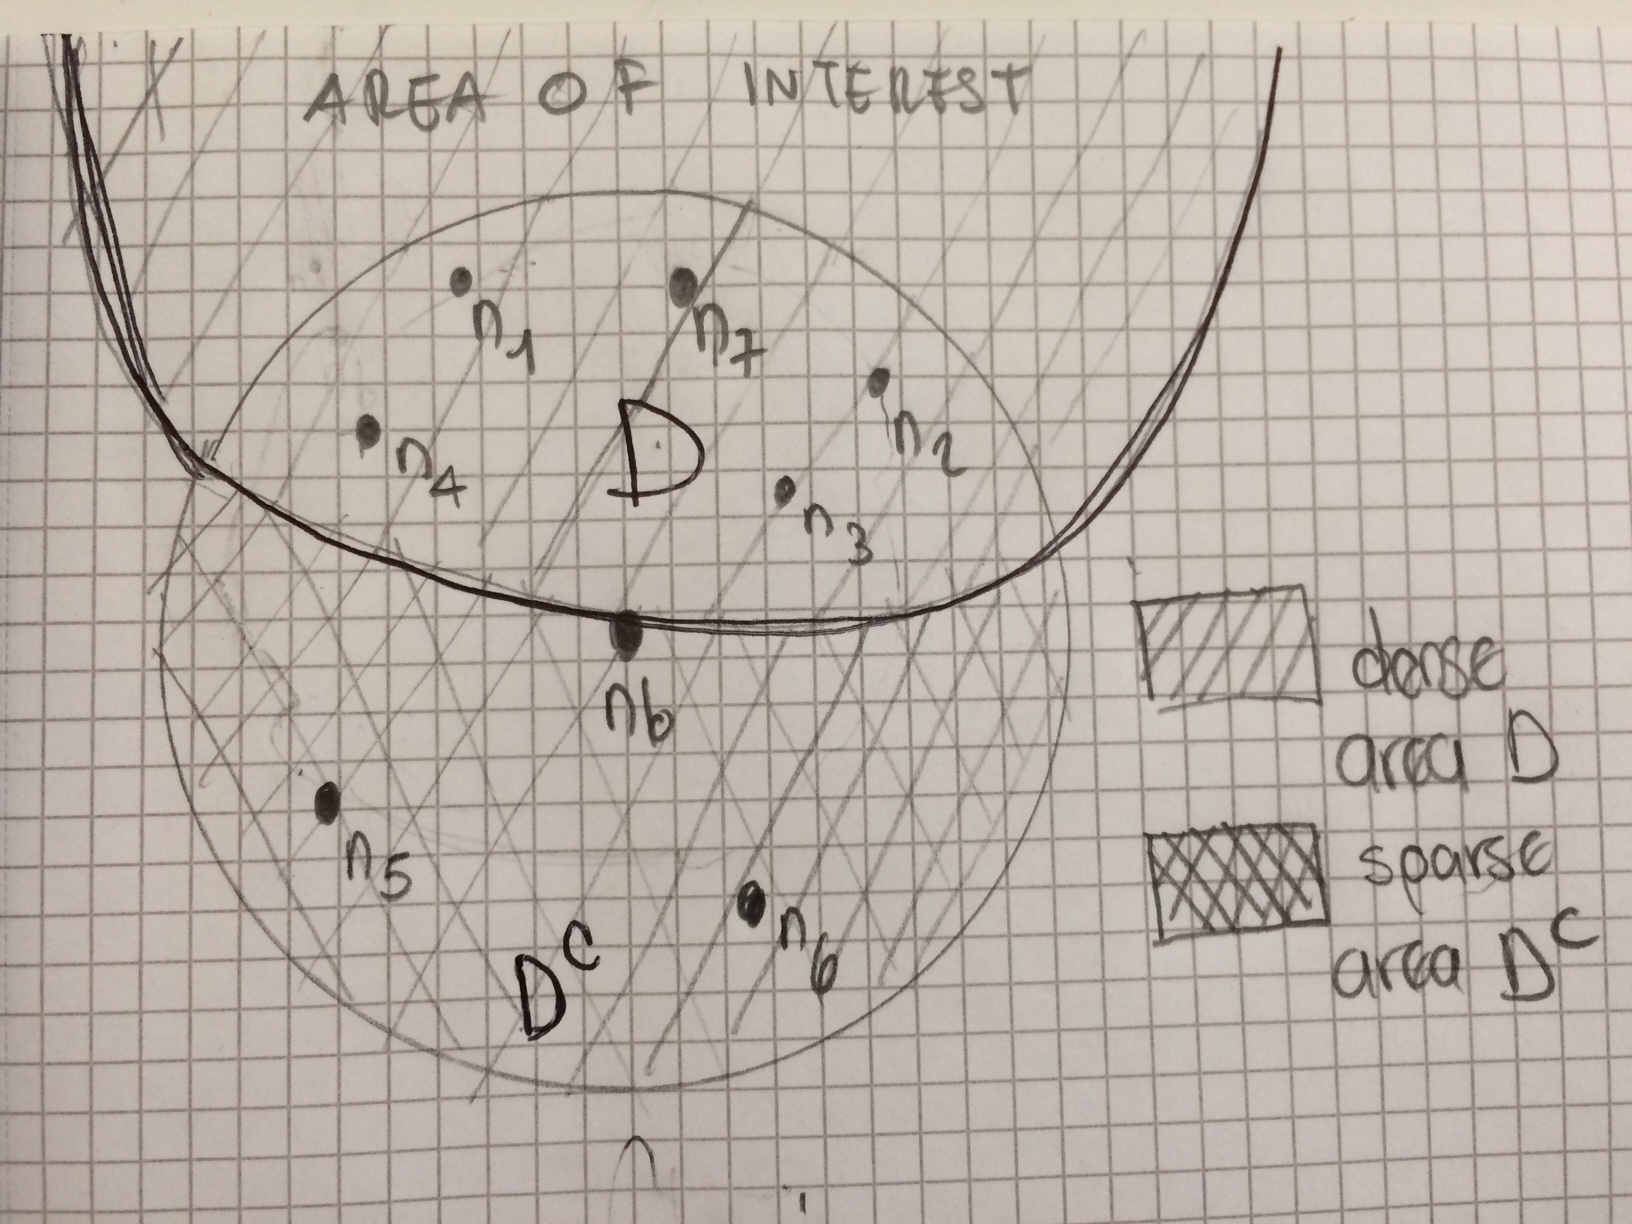
\includegraphics[scale=0.1]{figures/dense_sparse_region}
\caption{}
\label{fig:dense_sparse_region}
\end{figure}

\begin{figure}
\centering
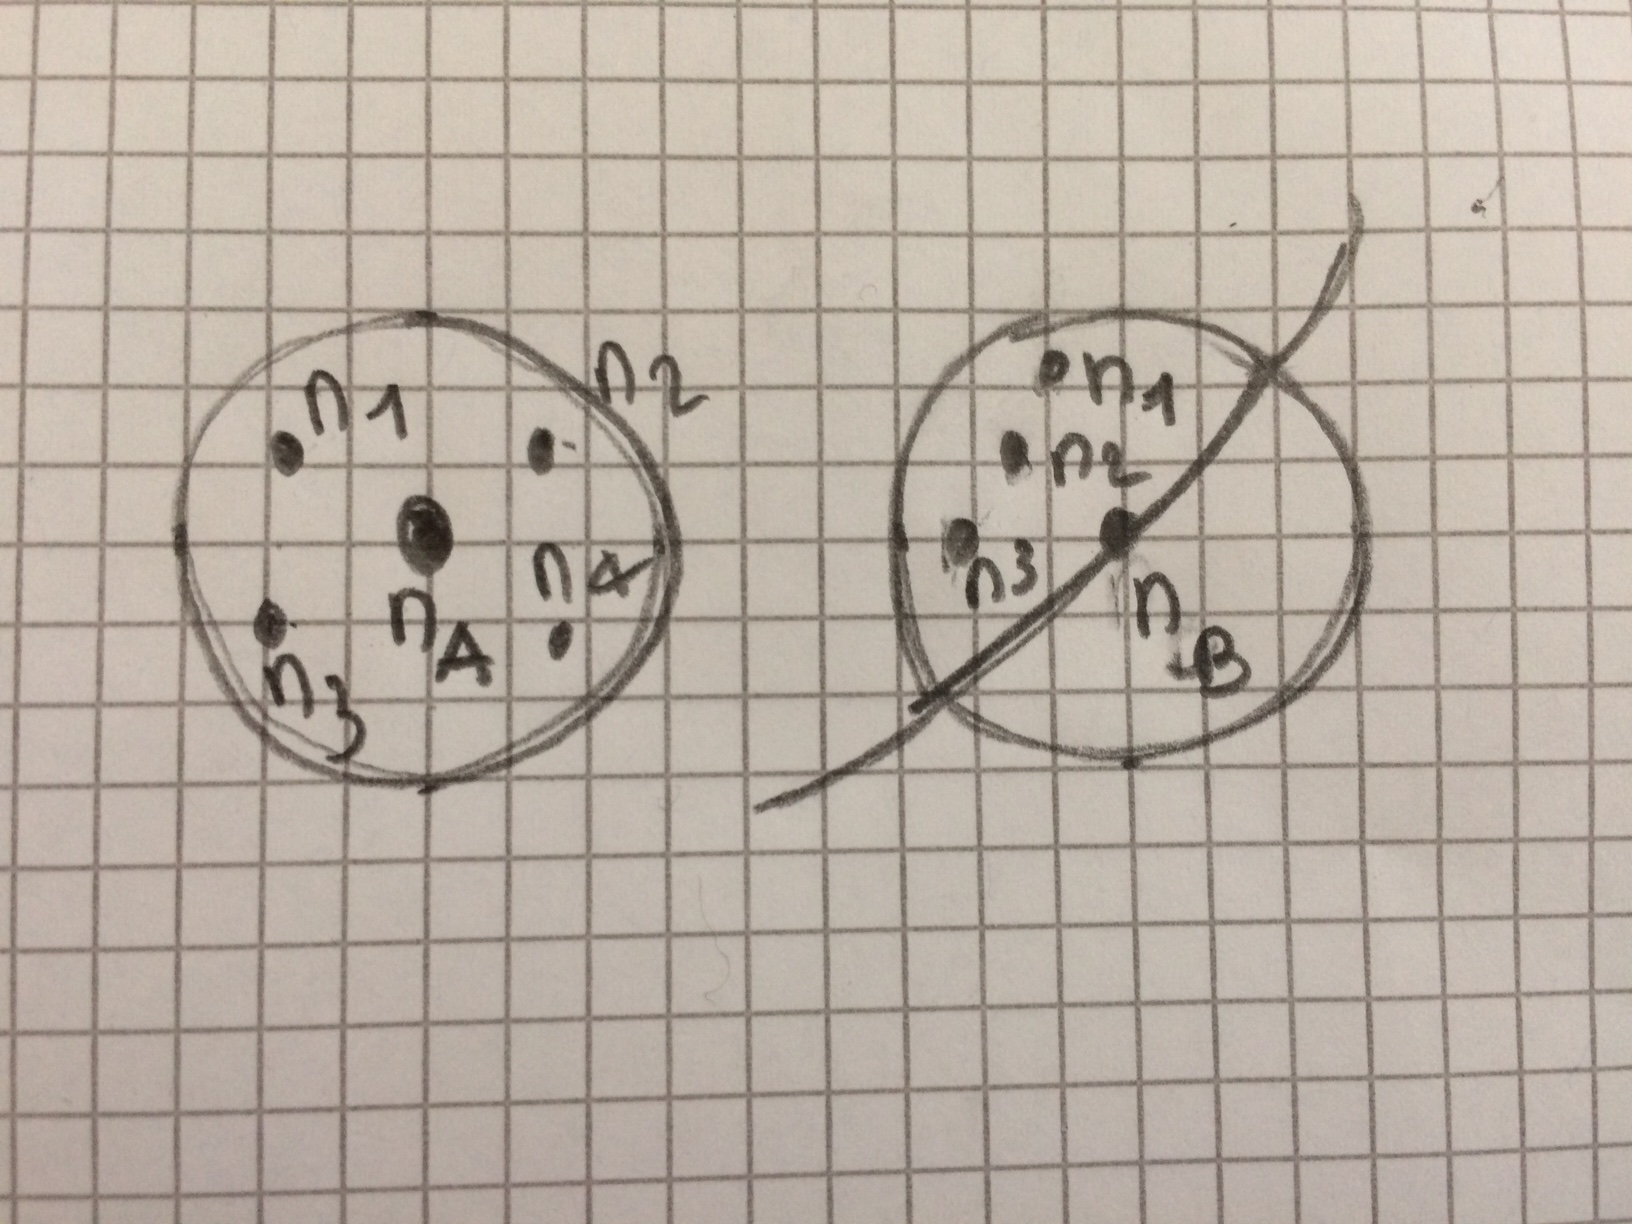
\includegraphics[scale=0.1]{figures/count_not_enough}
\caption{}
\label{fig:count_not_enough}
\end{figure}

\begin{figure}
\centering
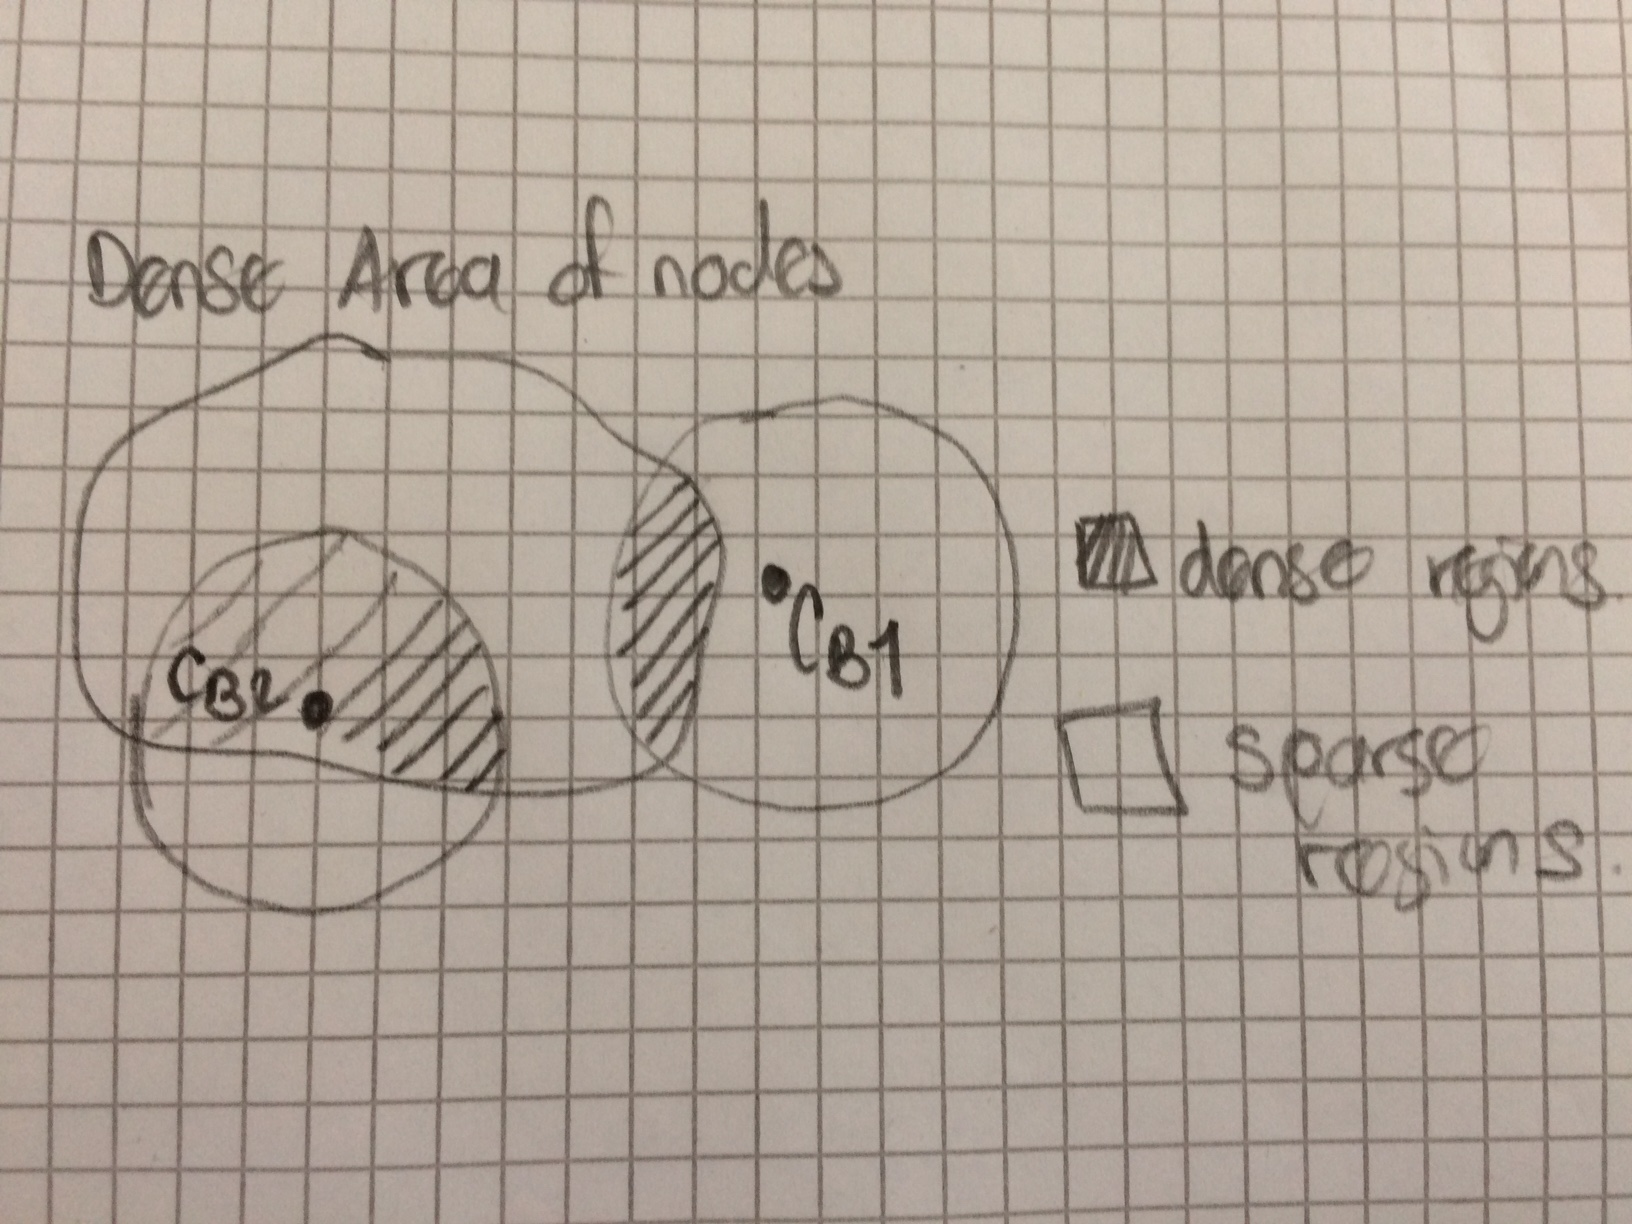
\includegraphics[scale=0.1]{figures/location_of_regions}
\caption{}
\label{fig:location_of_regions}
\end{figure}

\begin{figure}
\centering
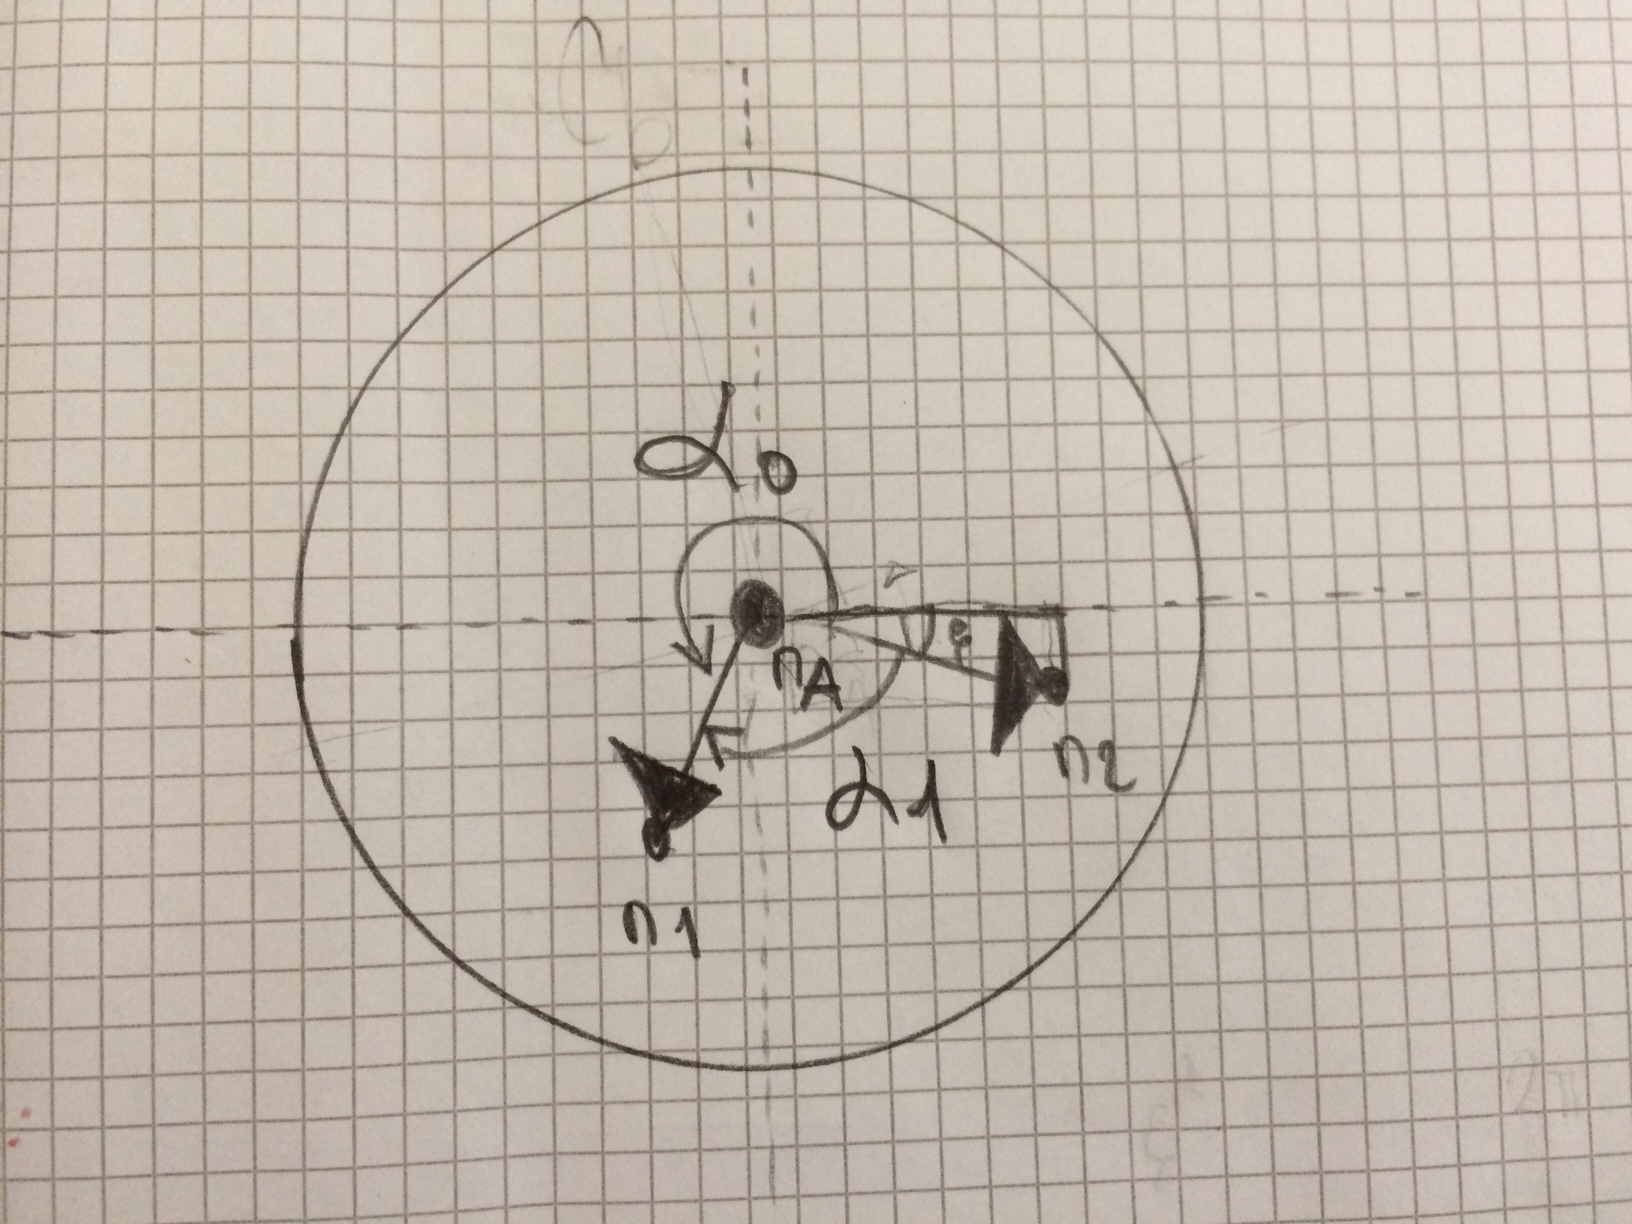
\includegraphics[scale=0.1]{figures/scenario1}
\caption{}
\label{fig:scenario1}
\end{figure}

\begin{figure}
\centering
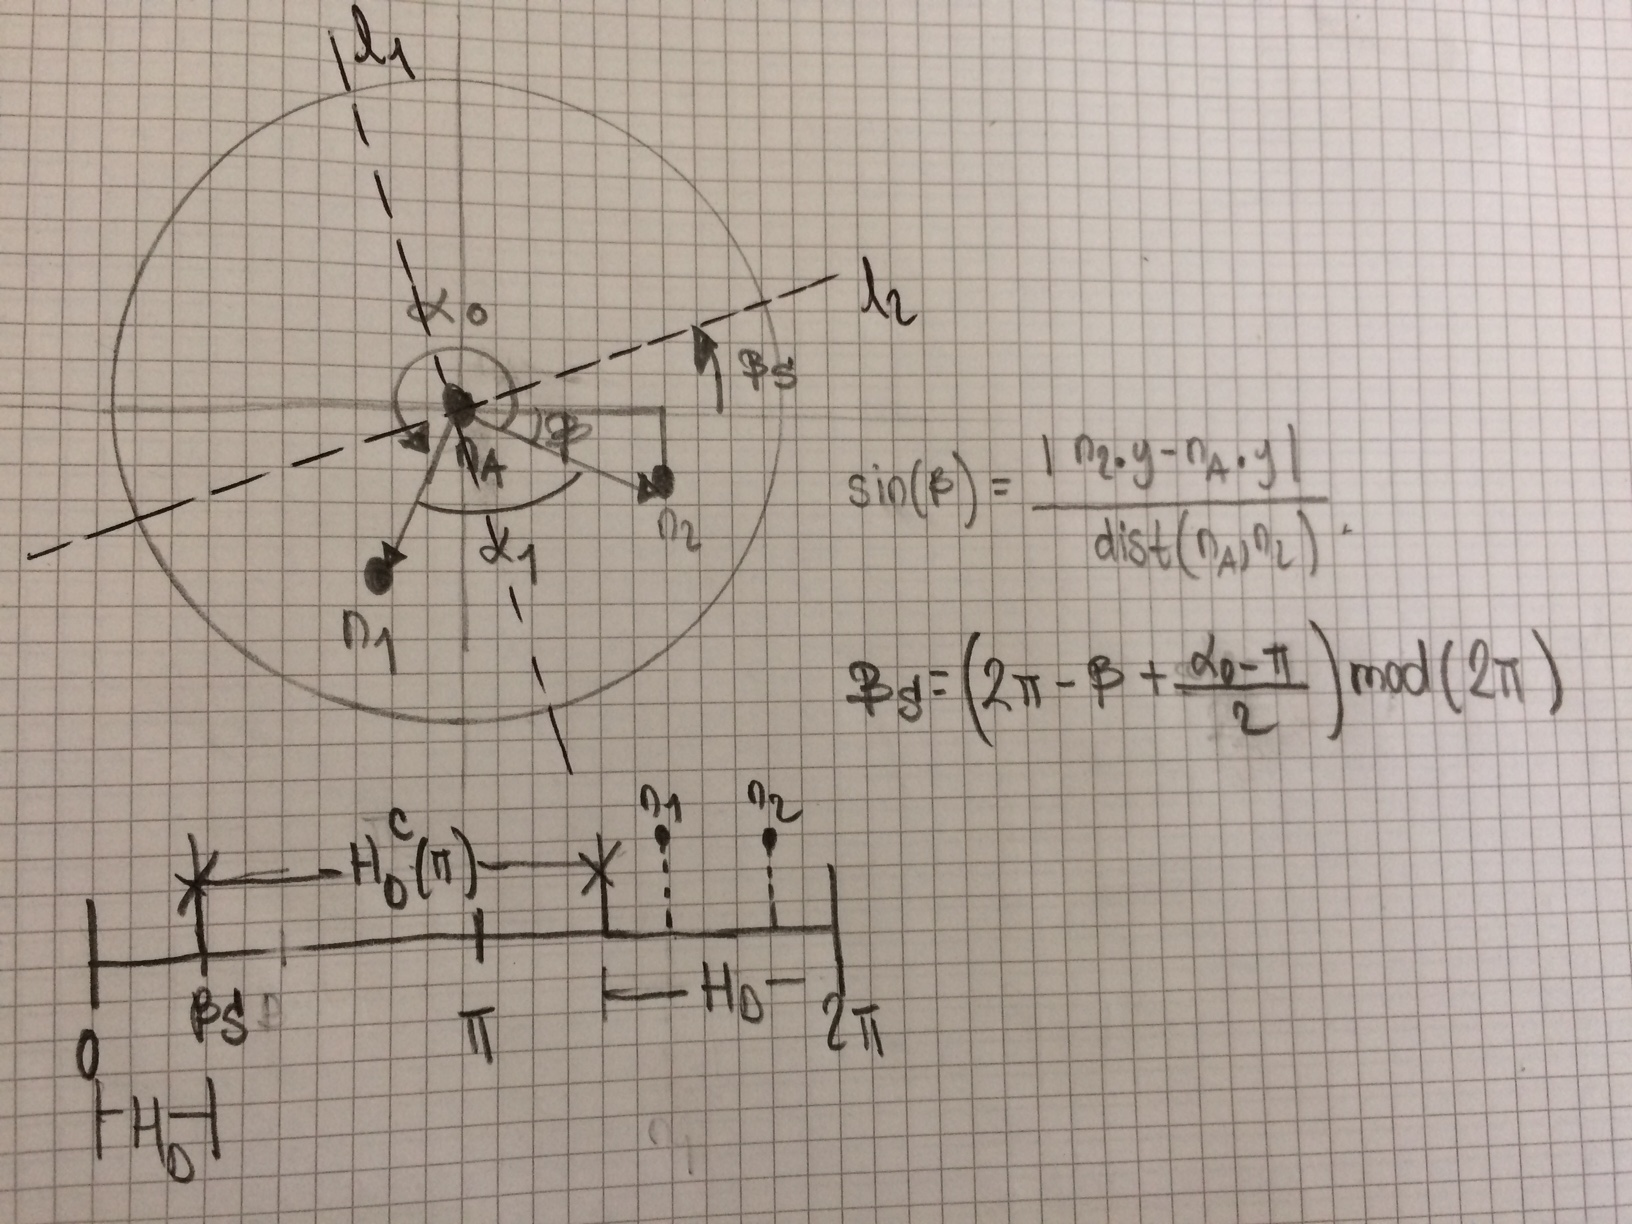
\includegraphics[scale=0.1]{figures/dense_disk_scenario1}
\caption{}
\label{fig:dense_disk_scenario1}
\end{figure}

\subsection{Location-based adaptation policy}
%
This adaptation policy labels those nodes located at the border of dense regions, which we call \emph{border nodes}.
%
When nodes move towards a preferred location, border nodes surround this location and we can characterize that the density within their area of transmission follows a bimodal distribution.
%
Let be $n_{b}$ a border node and $C_{b}$ its area of transmission, we can describe $C_{b}$ as a circle of radius $T_{x}$ centers at the position of $n_{b}$.
%
As shown in figure~\ref{fig:dense_sparse_region}, region $D$ within $C_{b}$ contains more nodes or is more dense than its complement $D^{c}$.
%
Our adaptation policy takes advantage of this systematic behavior of border nodes and uses the GPS coordinates, shared by any location-based broadcast algorithm, to tell nodes within a preferred location area when to start using an overlay-based approach.
%
The reasoning behind the construction of a virtual backbone is to benefit from the stationary conditions observed in a preferred location, nodes stay in such a location or tend to move all together towards a common direction.
%
We confirm a better utilization of nodes resources using an overlay-based solution within preferred locations in our experimental results.

\subsubsection{Characterization of border nodes' transmission area}
A node in the network will be labeled as border node if one half of its area of communication $C_{b}$ contains at least $d$ nodes, where the threshold $d$ is a fixed parameter and it is part of our adaptation layer (see figure~\ref{}). \raziel{give an argument about the 50, 50 approach}
%
As depicted in figure~\ref{fig:count_not_enough}, counting the number of neighbors within the communication area of nodes is not enough, we have to find the region $H_{D}$ with at least $d$ nodes such that its sparse complement $H_{D}^{C}$ contains less than $d-1$ nodes.
%
The orientation of such $H_{D}$ is a concern too, as figure~\ref{fig:location_of_regions} depicts, the most dense region in $C_{B1}$ points towards west while $C_{B2}$ points to north.
\raziel{here you need a comment about what branch in math study this kind of problems. Continue digging into: gauss circle problem, minimal enclosing circle, circle packing, spatial analysis, etc...}

Let us consider how to find $H_{D}$ in a scenario where one node has two neighbors.
%
As figure~\ref{fig:scenario1} shows, we observe that $\alpha_{0}$ is the biggest angle with a size in radians equal to $\alpha_{0} = 2\pi - \measuredangle n_{2}n_{A}n_{1}$. Given $\alpha_{0} > \pi$ there exist an infinite number of half disks with an sparse density within $\alpha_{0}$.
%
For our proposes, it is enough to define just one sparse region $H_{D}^{C}$ of $\pi$ radians.
%
In order to find $H_{D}^{C}$ we split $\alpha_{0}$ in two equal parts by drawing a line $l_{1}$ at the middle of $\alpha_{0}$ crossing the position of node $n_{A}$, as figure~\ref{fig:dense_disk_scenario1} depicts.


\raziel{
\textbf{Cost of control messages}
Control messages serve to fetch fresh information about nodes' surroundings with the aim of deciding when to forward broadcast messages.
Control messages are critical in the latest adaptive-based techniques to broadcast in homogeneous MANET's ~\cite{hypergossiping, ProbFlood} \raziel{If you like the idea, add more reference to adaptive-based approaches, otherwise, to contradict this idea feel free to reference works where adaptation takes place without the use of control messages}.
However, these techniques perform a pure flooding approach in a periodic way to disseminate control messages.
As a result, \emph{storms of broadcast and control messages} reduces network coverage \raziel{I propose to rename "network coverage" as "reachability", the latter has been used by the community in seminal works ~\cite{hypergossiping, BroadcastStormProblem}. Reachability will give us the proportion of nodes that successfully received a broadcast message in all partitions of our experimental scenario. Or, we can keep add "reachability" to our list of broadcast metrics.}
In \OurAdaptiveTech, we propose the use of a beacon-less technique (\raziel{An augmented version of ABBA where timers are inversely proportional to nodes' density. Particularly, we are interested in maintaining the list of neighbors on each node. Additionally, the upper-bounds values to set timers can be dynamically changed too for speeding-up the dissemination time; this is important when a switch of context take place.}) to disseminate control messages with the aim of having updated lists of nodes' neighbors. We formulate the next hypothesis: \textbf{the overall energy consumption of nodes used by a the periodic simple-flooding technique to disseminate control messages is bigger than the cost of control messages dissemination with ABBA $+$ $f_{GPS}(N)$}, where $f_{GPS}$ approximates the cost of fetching $N$' GPS coordinates periodically. This frequency is proportional to $N$ velocity (\raziel{we can gather this information from mobile's accelerometer}). This will require a deep analysis in ABBA (\raziel{in form a table to map the inpact in our broadcast metrics and the different tunes of ABBA}).
\paragraph{Drawbacks} ABBA requires nodes position to its functioning. 
\textbf{Brainstorming}
\paragraph{Ideas to ameliorate cost of localization}
This work~\cite{enloc} ameliorates the energy cost of getting localization of nodes.
Current adaptive solutions change the value of thresholds to be well informed before performing message retransmissions.
\paragraph{Some questions to consider in adaptation:}
\begin{itemize}
	\item How to get a fresh list of nodes' neighbors?
	\item When to perform a switch of context (change of algorithm)?
	\item How to disseminate SWITCH\_OF\_CONTEXT messages?
\end{itemize}
}